\documentclass[12pt,a4paper]{article}

% Margins.
\setlength{\oddsidemargin}{0in}
\setlength{\evensidemargin}{0in}
\setlength{\headheight}{12pt}
\setlength{\headsep}{42pt}
\setlength{\topmargin}{-54pt}
\setlength{\textwidth}{6.5in}
\setlength{\textheight}{10in}

\usepackage{amsmath}
\usepackage{float}
\usepackage{graphicx}
\usepackage[hyphens]{url}
\usepackage{hyperref}	% Clickable links to figures, references and urls.
\usepackage{datetime}
\usepackage{longtable}
\usepackage{subfigure}

% Links direct to top of figures.
\usepackage[all]{hypcap}

% Drawing.
\usepackage{pgf}
\usepackage{tikz}

% Listings for formatting code.
\usepackage{listings}
\usepackage{textcomp}
% General options.+++
\lstset{breaklines=true, basicstyle=\small\ttfamily, tabsize=4, numbers=left, stepnumber=1, frame=single, showstringspaces=false, upquote=true}
% C++ specific high-lighting. Comments are 50/50 shades of green/black and strings coloured with 60/40 red/black mixture.
\lstset{language=[ISO]C++, commentstyle=\color{green!50!black}, keywordstyle=\color{blue}, stringstyle=\color{red!60!black}}

%opening
\title{\vspace{-3cm}Physics for Engineers\\Class 23\\Gauss's Law: Applications I}
\author{Attique Dawood}
\date{March 17, 2014\\[0.2cm] Last Modified: \today, \currenttime}
\begin{document}
\maketitle
\section{Announcements}
\begin{itemize}
\item None.
\end{itemize}
\section{Revision}
\begin{itemize}
\item Gauss's Law.
\end{itemize}
\section{Exercises}
\noindent\textbf{Question 1:} Use Gauss's Law to find electric field of an infinite line charge with uniform charge density $\rho_L$ placed along $z$--axis.\\[0.2cm]
\noindent\textbf{Question 2:} A spherical charge distribution with uniform charge density $\rho_v$ and radius $R$ exists centred at origin. Use Gauss's Law to find electric field everywhere.\\[0.2cm]
\noindent\textbf{Question 3:} Use Gauss's Law to find the electric field of an infinite sheet of charge with a uniform charge density $\rho_S$.\\[0.2cm]
\noindent\textbf{Question 4:} A uniform charge density $\rho_v$ exists in the region from $r=a$ to $r=b$. Find electric field everywhere.\\[0.2cm]
%\begin{itemize}
%\item[a.] Electric field of a point charge.
%\item[b.] Electric field of an infinite line charge placed along $z$--axis.
%\end{itemize}
%%\begin{figure}[H]
%\centering
%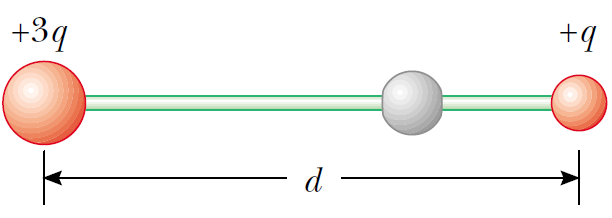
\includegraphics[scale=0.45]{FigureP23-10.png}
%\caption{Equilibrium of charge.}
%\label{Equilibrium}
%\end{figure}
%\nocite{*}
%\bibliographystyle{plain}
%\bibliography{PhysicsRef}
\end{document}
